\section{Advanced thermophysical model for rough surface including craters}
\label{sec:5}

This section shows the implementation of the self heating. A normal at the surface of an asteroid may appear to be hidden from the direct solar flux even if it is situated in the day side, for instance inside a crater. In this scenario, it is important to take into consideration what is called the self heating of the asteroid. Due to its albedo, the surface of the asteroid relfects sunlight rays and thus, if the asteroid is not purely smooth, some reflected rays might impact another location on the asteroid resulting in heating it up.

\subsection{Theory}

\begin{figure*}[b]
    \centering
    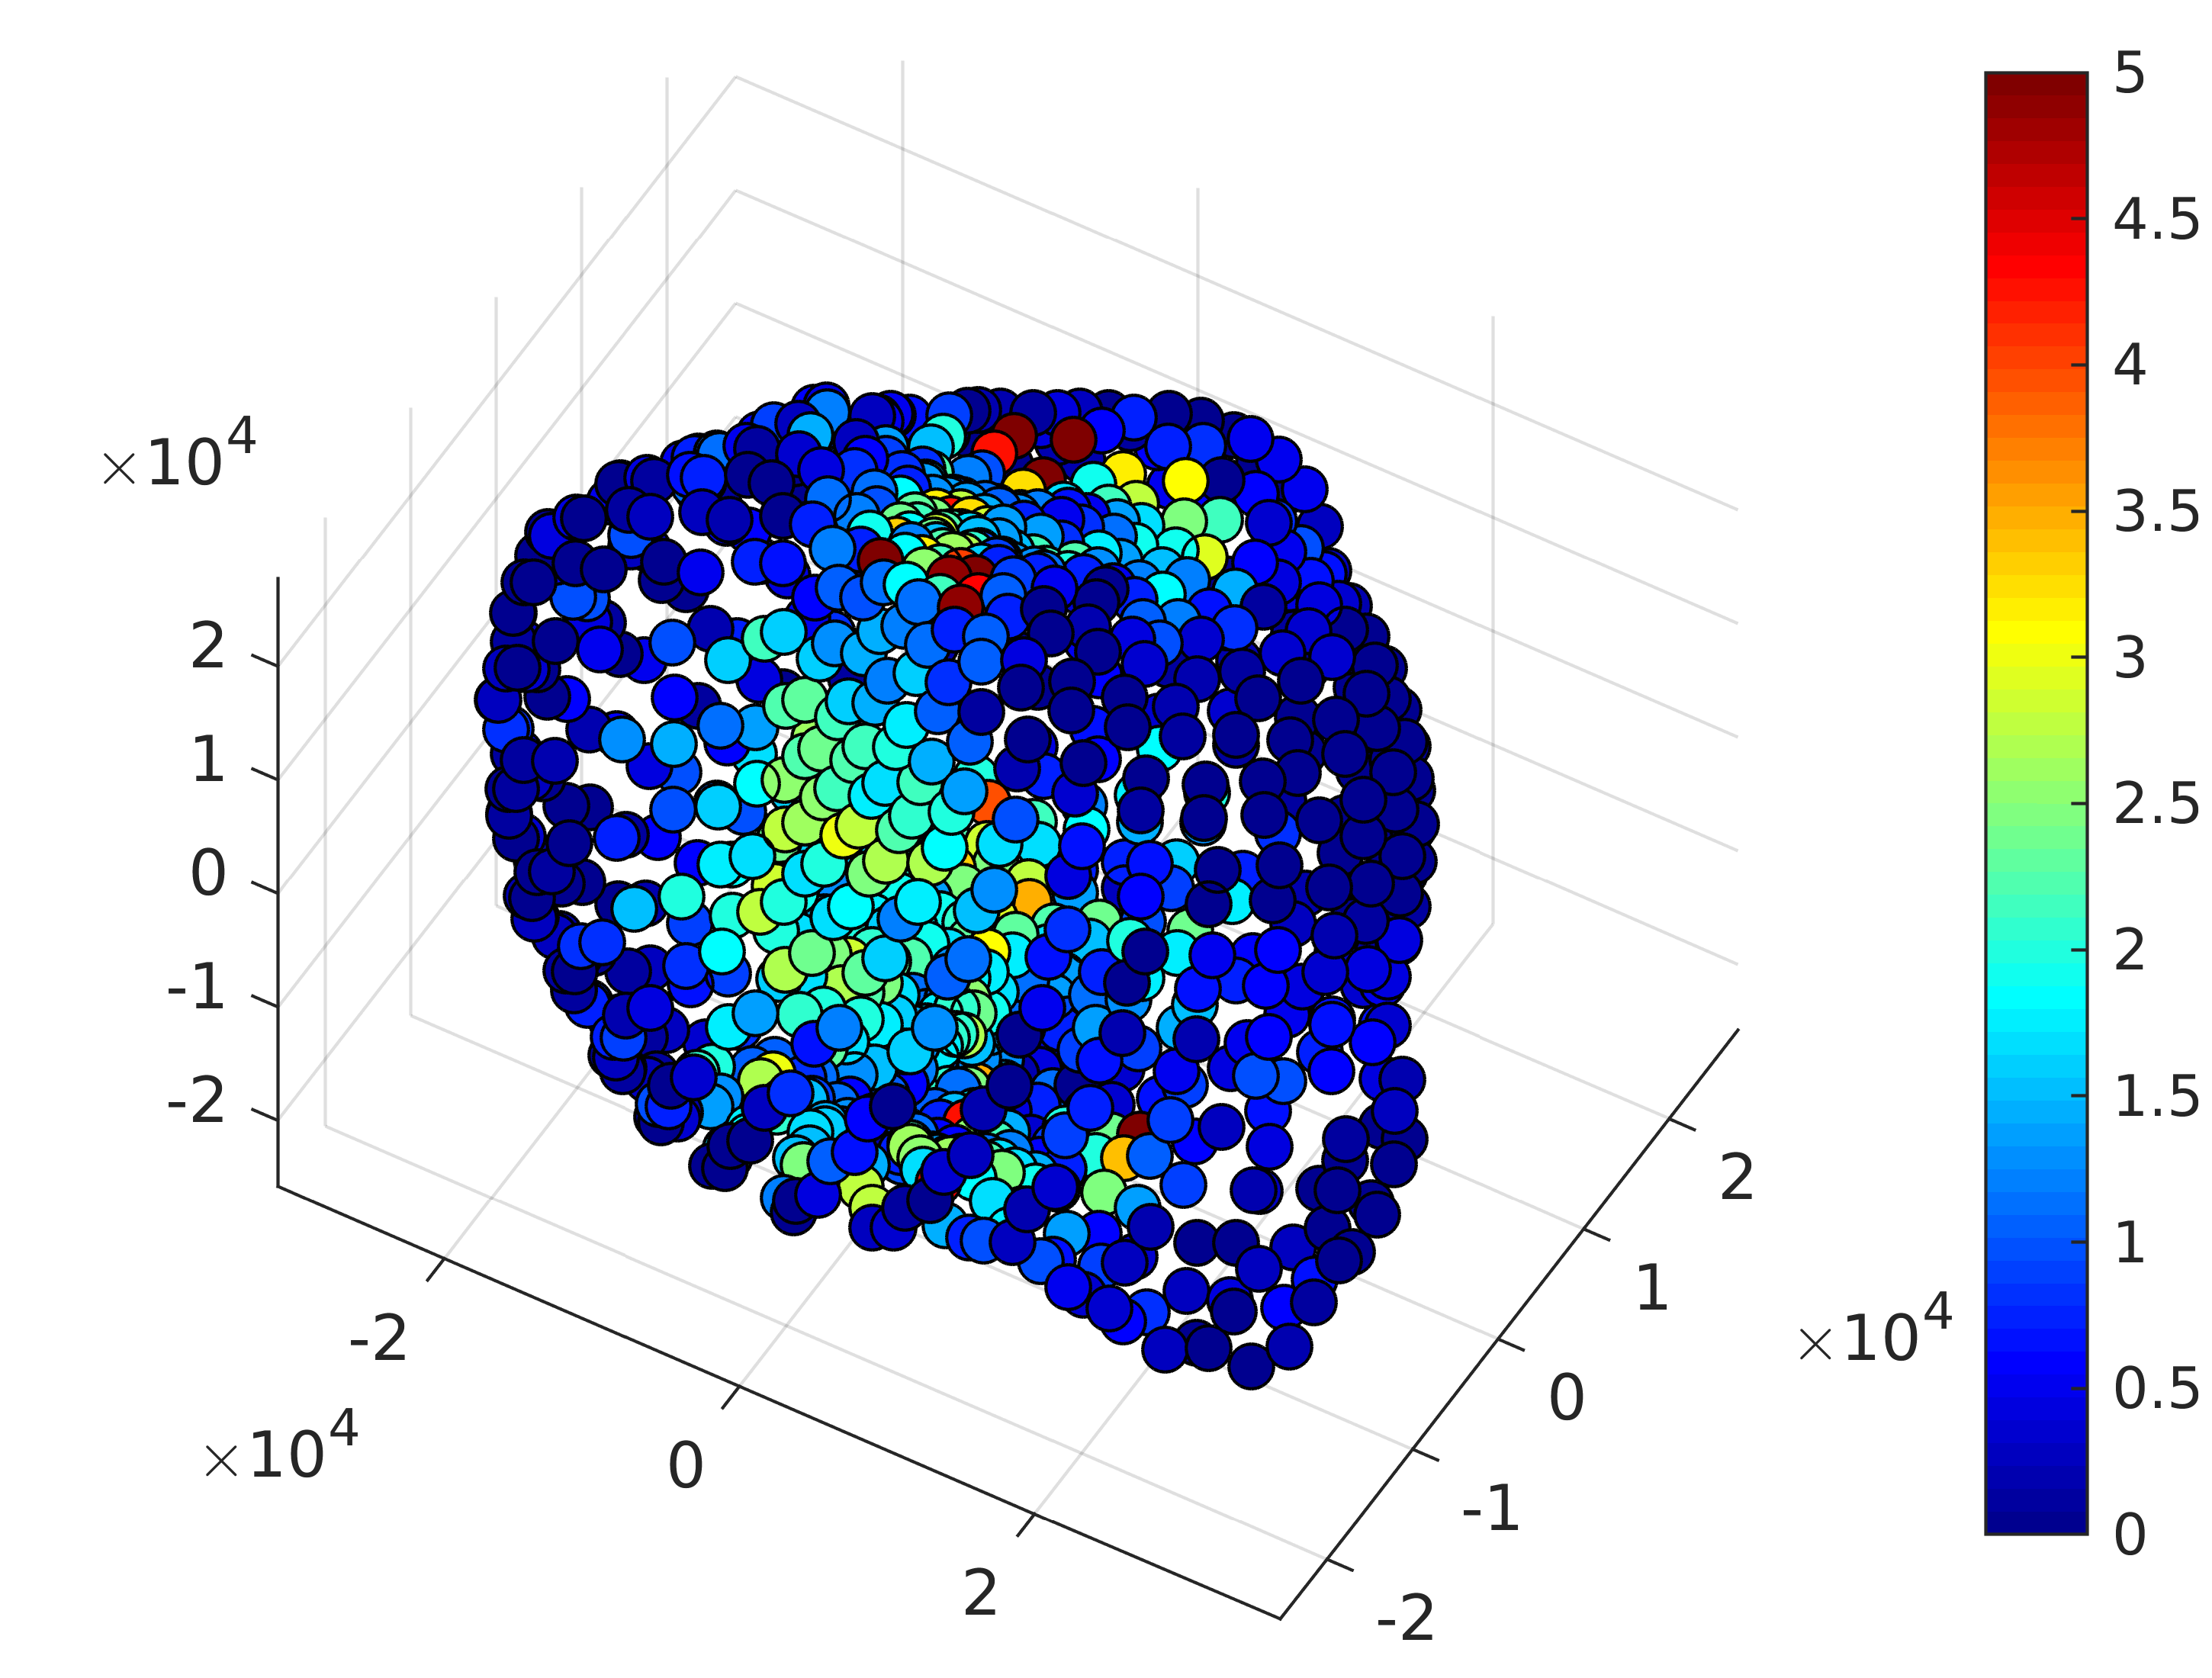
\includegraphics[width=0.33\linewidth]{rsc/self_3D_1.png}
    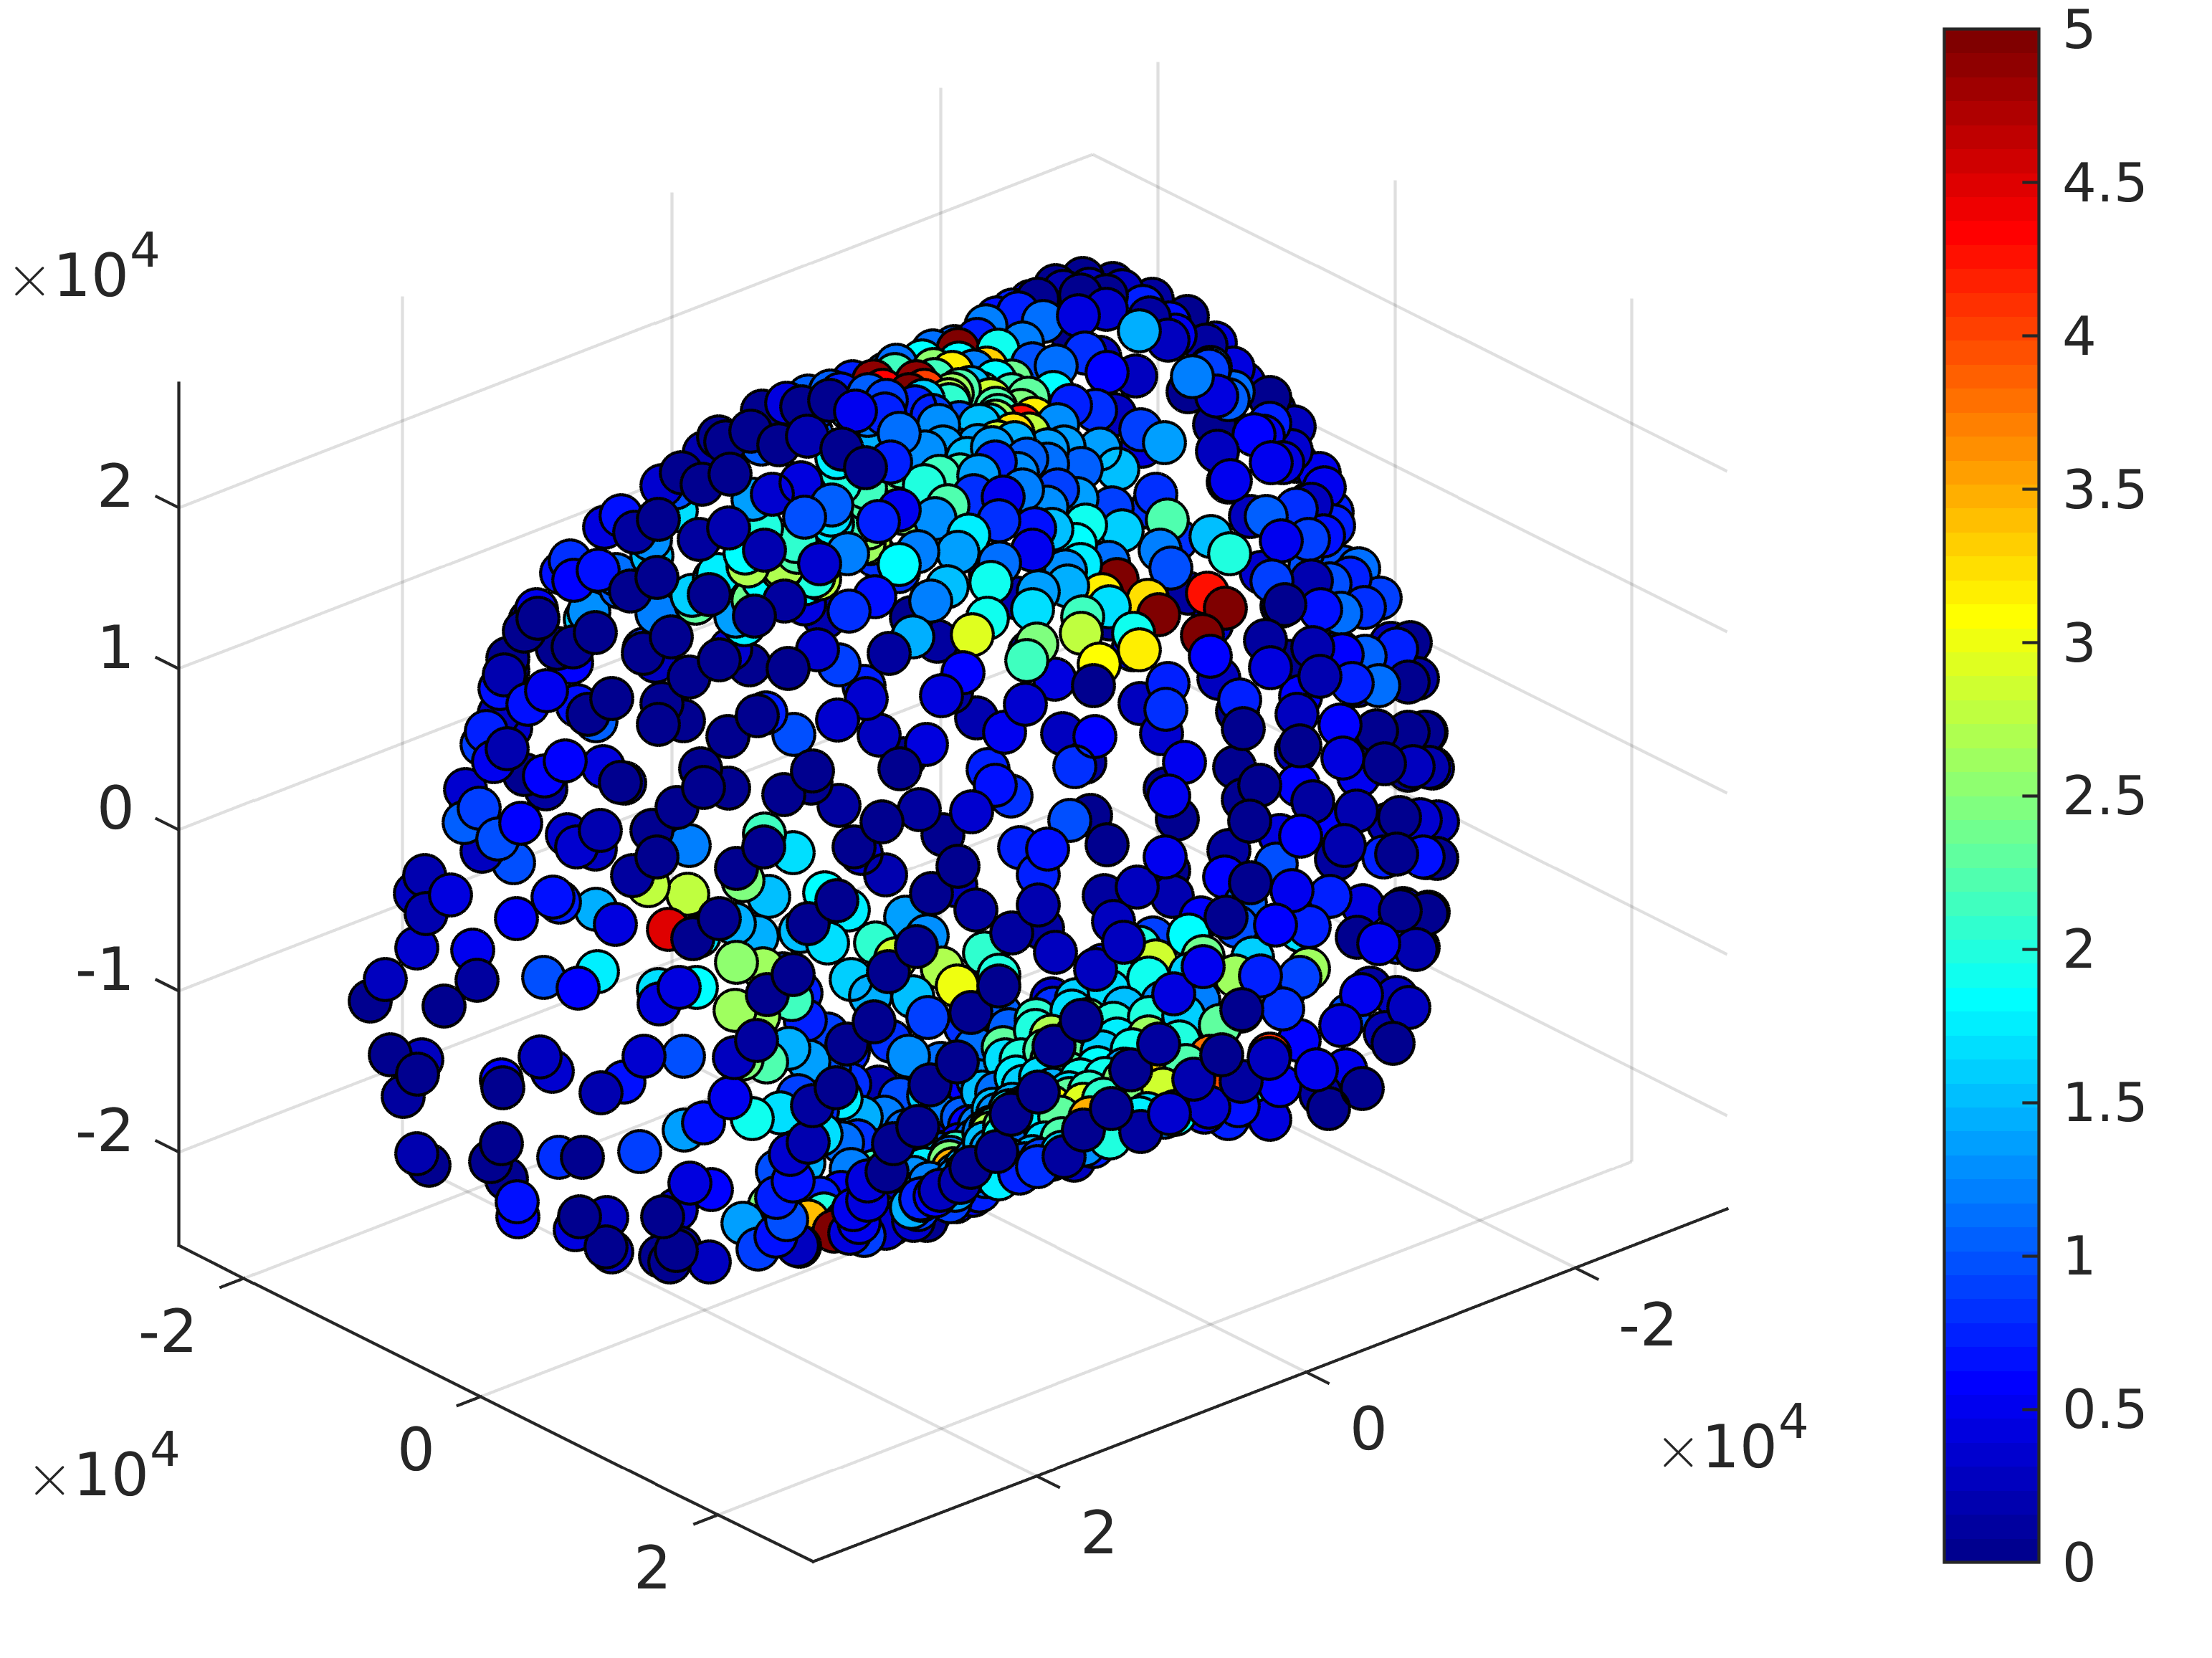
\includegraphics[width=0.33\linewidth]{rsc/self_3D_2.png}
    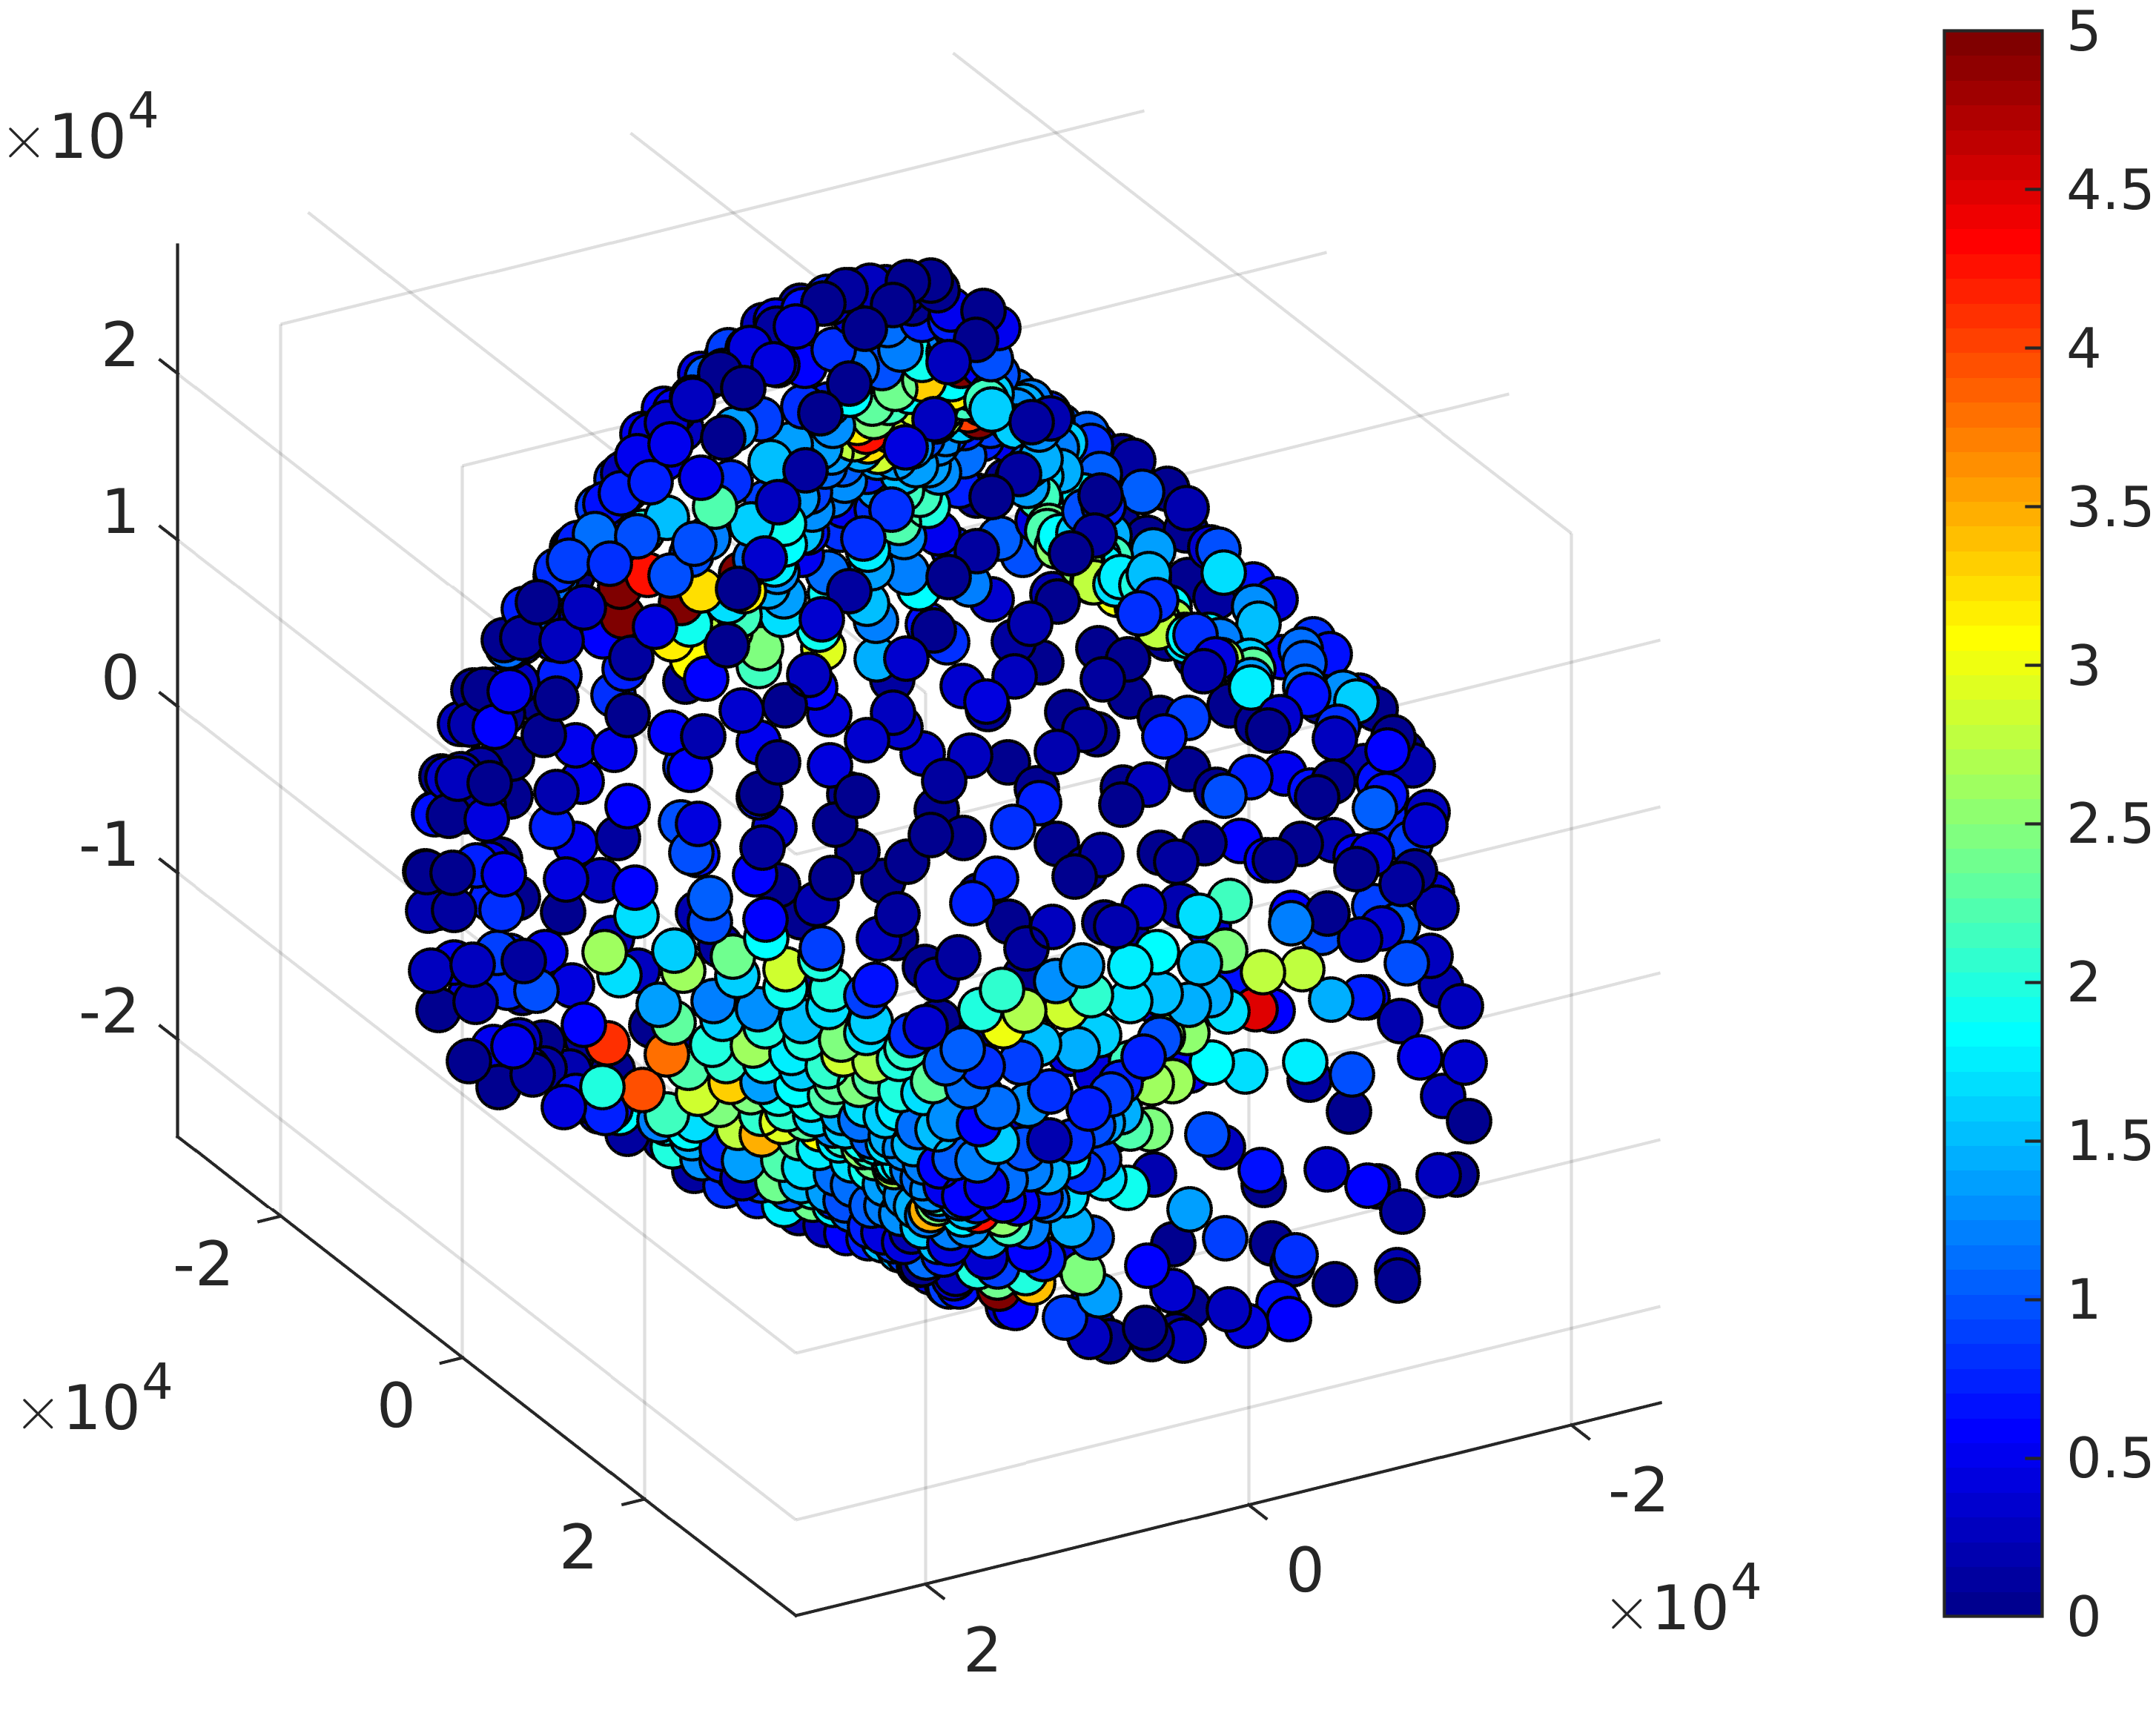
\includegraphics[width=0.33\linewidth]{rsc/self_3D_3.png}
    \caption{Self heating contribution displayed on the 3D shape model of the asteroid Mathilde.}
    \label{fig:5.5}
\end{figure*}

The implementation of the thermophysical model beaming into Didymoon, described in \autoref{sec:4}, had mutual-heating occurring between the two bodies of the Didymos system. However, this implementation neglected global self heating that can occur within large-scale concavities of an irregularly shaped asteroid.

Global self-heating provides a mechanism for heat to be transferred laterally across an asteroid surface. \autoref{fig:5.5} demonstrates how global self heating can affect the thermophysical model and temperatures predictions for an asteroid with a large-scale concavity and an irregular shape. The large-scale concavity results in heat transfers that occur at certain geometries, where a facet is facing another one. In the absence of global self heating, those facets would receive only direct flux and mutual heating flux. However, if the facet receives reflected solar flux and emitted thermal radiation from the opposite side of the concavity that is illuminated, the temperature would be higher than expected. The aim of this section is to implement this phenomenon.

\begin{center}
    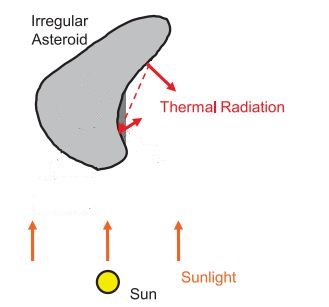
\includegraphics[width=0.5\linewidth]{rsc/self.jpg}
    \captionof{figure}{Schematic of global self-heating occurring inside a large concavity of an asteroid.}
    \label{fig:5.1}
\end{center}

In the specific case of Didymoon, its shape model is still incredibly simple. The ESA's shape for Didymoon is a smooth ellipsoid. This leads in the total absence of self heating. For this purpose, a more complex shape model has been taken, Mathilde, visible in \autoref{fig:5.2}.
\begin{center}
    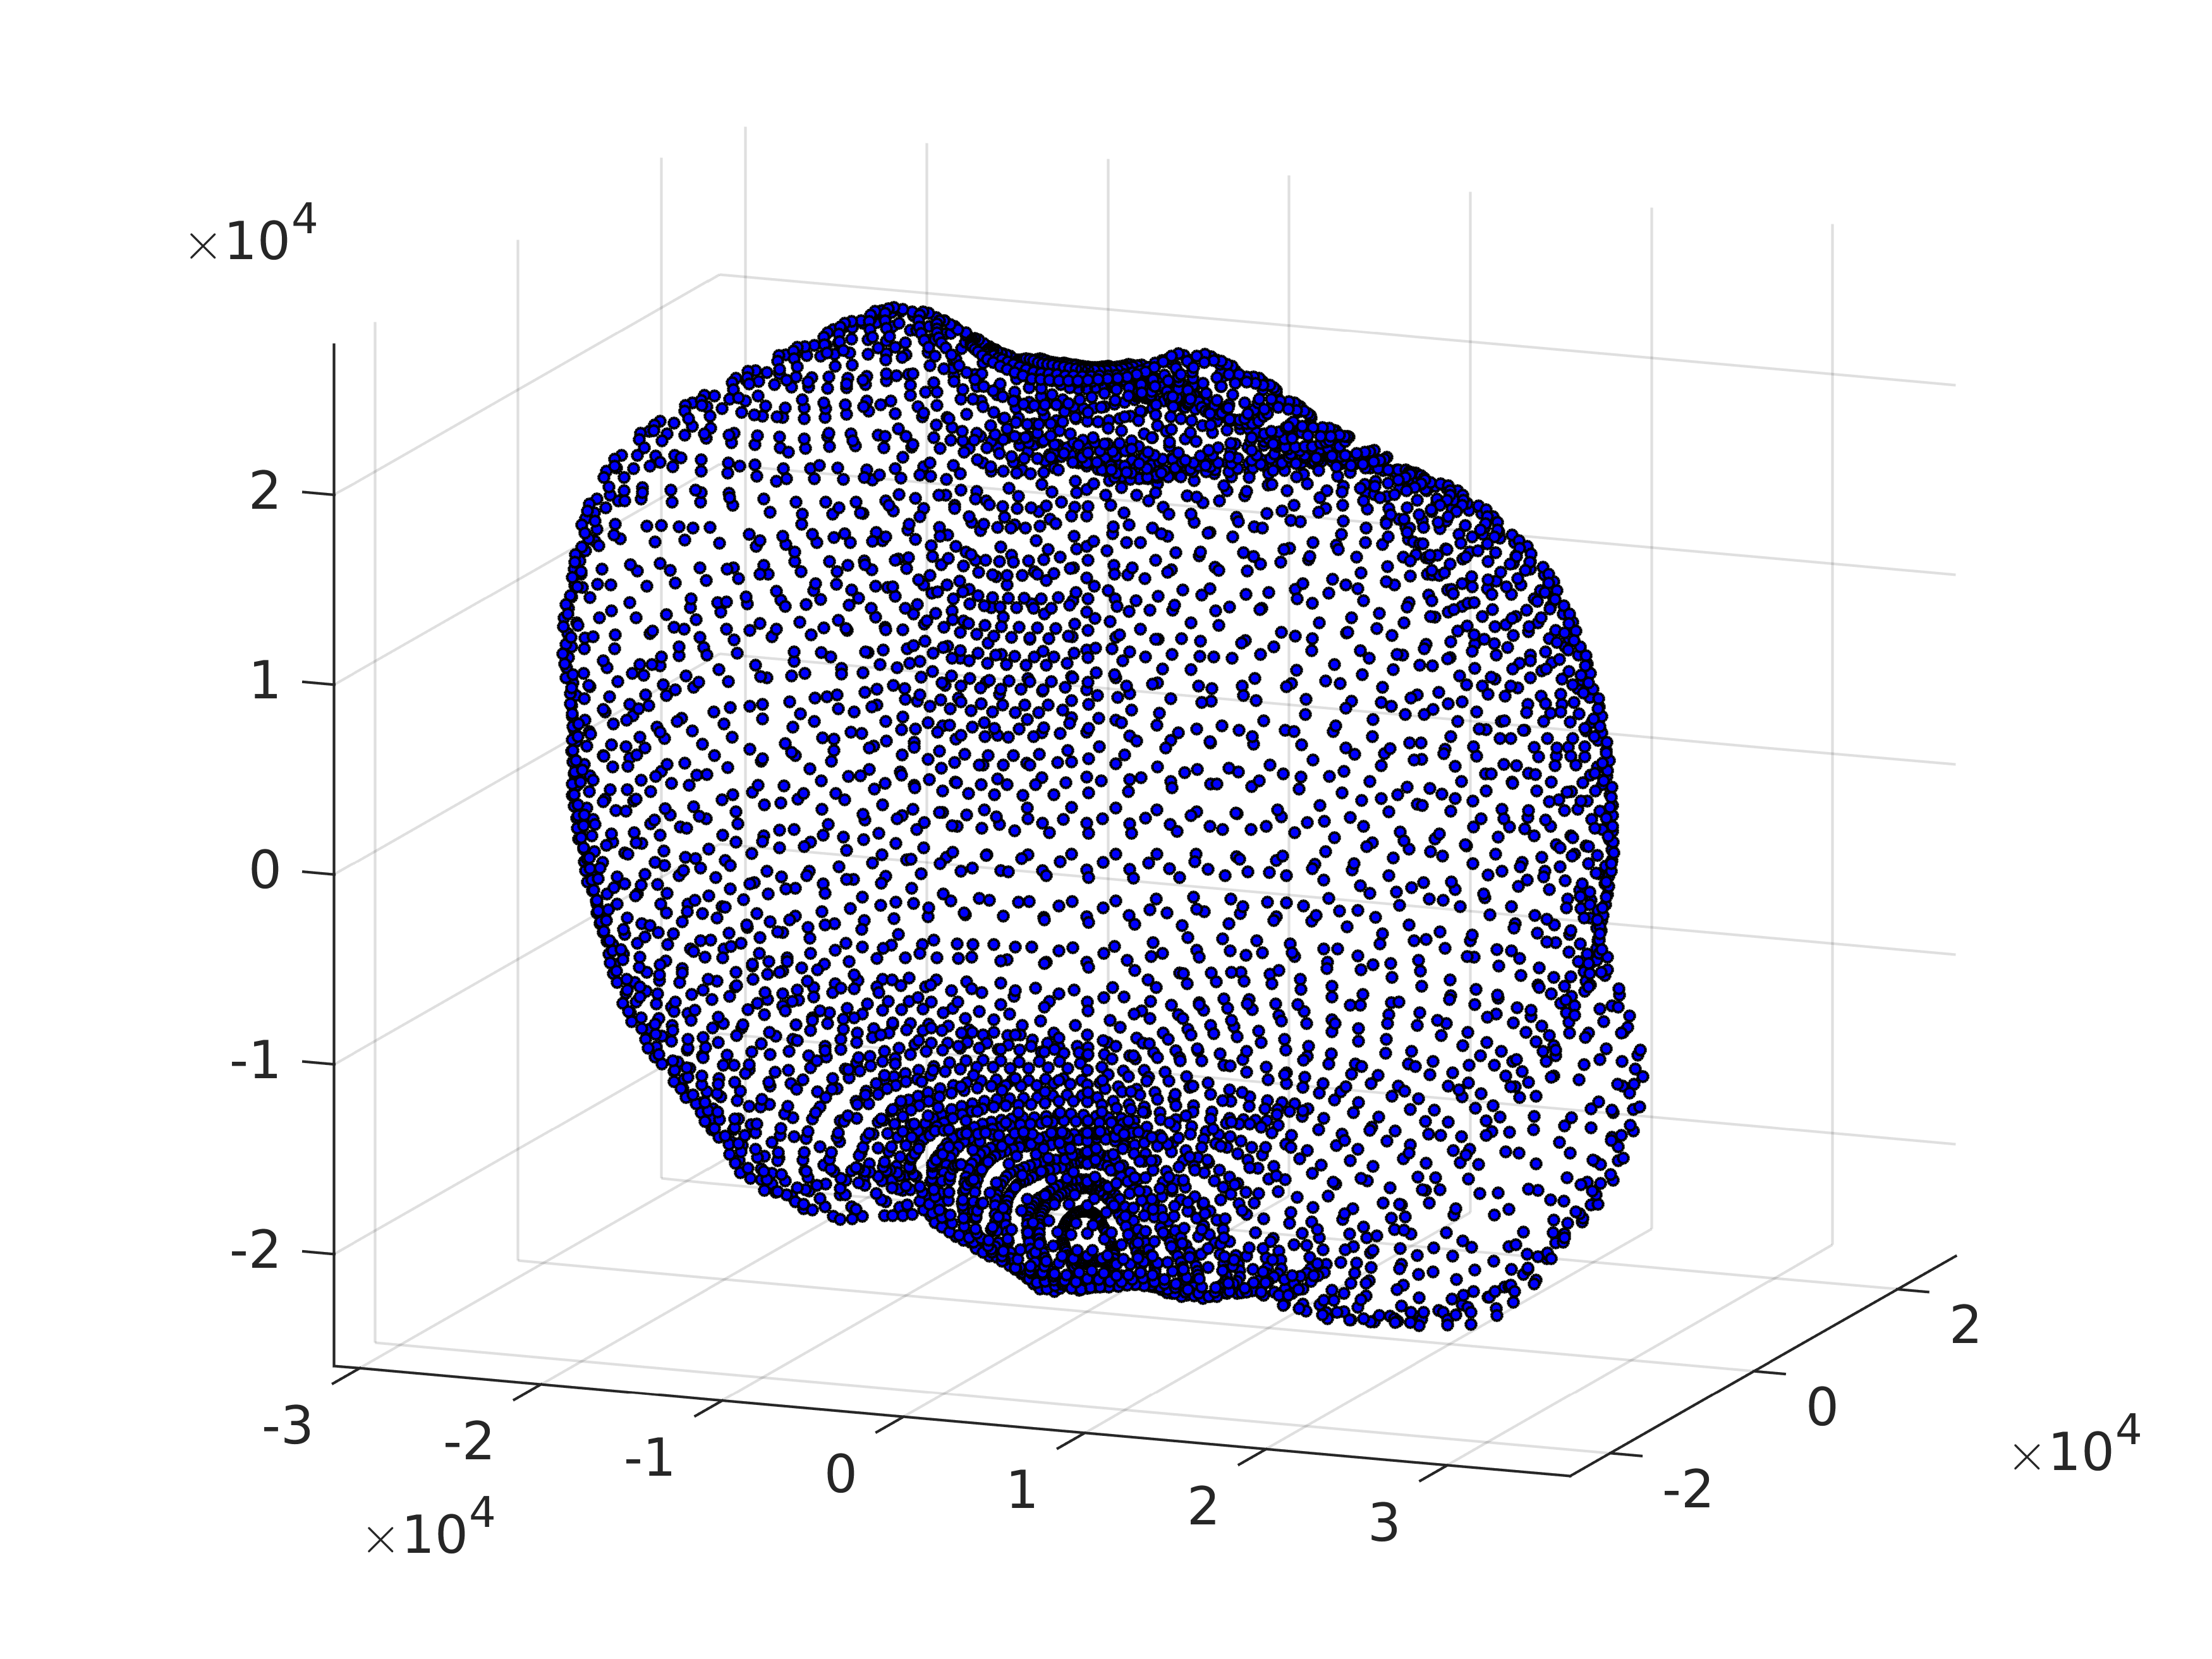
\includegraphics[width=0.7\linewidth]{rsc/mathilde.png}
    \captionof{figure}{Shape model of the asteroid Mathilde. Dimensions: 66x48x46 km.}
    \label{fig:5.2}
\end{center}

The two terms relative to the self heating in \autoref{eq:4.1} are now considered following:
\begin{equation}
    W_m=\sum_{i_1\neq i_2}^N V_{i_1i_2}\frac{S_{\odot}A\cos\varsigma_{i_2}}{r_H^2}
    \label{eq:5.1}
\end{equation}
\begin{equation}
    Q_m=\sum_{i_1\neq i_2}^N V_{i_1i_2}\epsilon\sigma u_{i_2}^4
    \label{eq:5.2}
\end{equation}
These two equations complete the model seen in \autoref{eq:4.1}. They are very similar to the mutual heating. The only difference is the indices of the facets. Each surface node temperature is computed with respect to every other node on the asteroid except the current one. $i_1$ and $i_2$ belong to the asteroid. $V_{i_1i_2}$ is computed as seen in \autoref{eq:4.3}. Same assumptions are made for $u_{i_2}$ as in the \autoref{sec:4}.

\subsection{Integration}
To investigate in general how global self heating within large concavities of asteroids influences thermophysical model, it is needed to first check the result's consistency, such as the surface temperature expected to be higher in a crater. The implementation of the self heating on the shape model of the asteroid Mathilde results in the thermal map in \autoref{fig:5.3}.
\begin{center}
    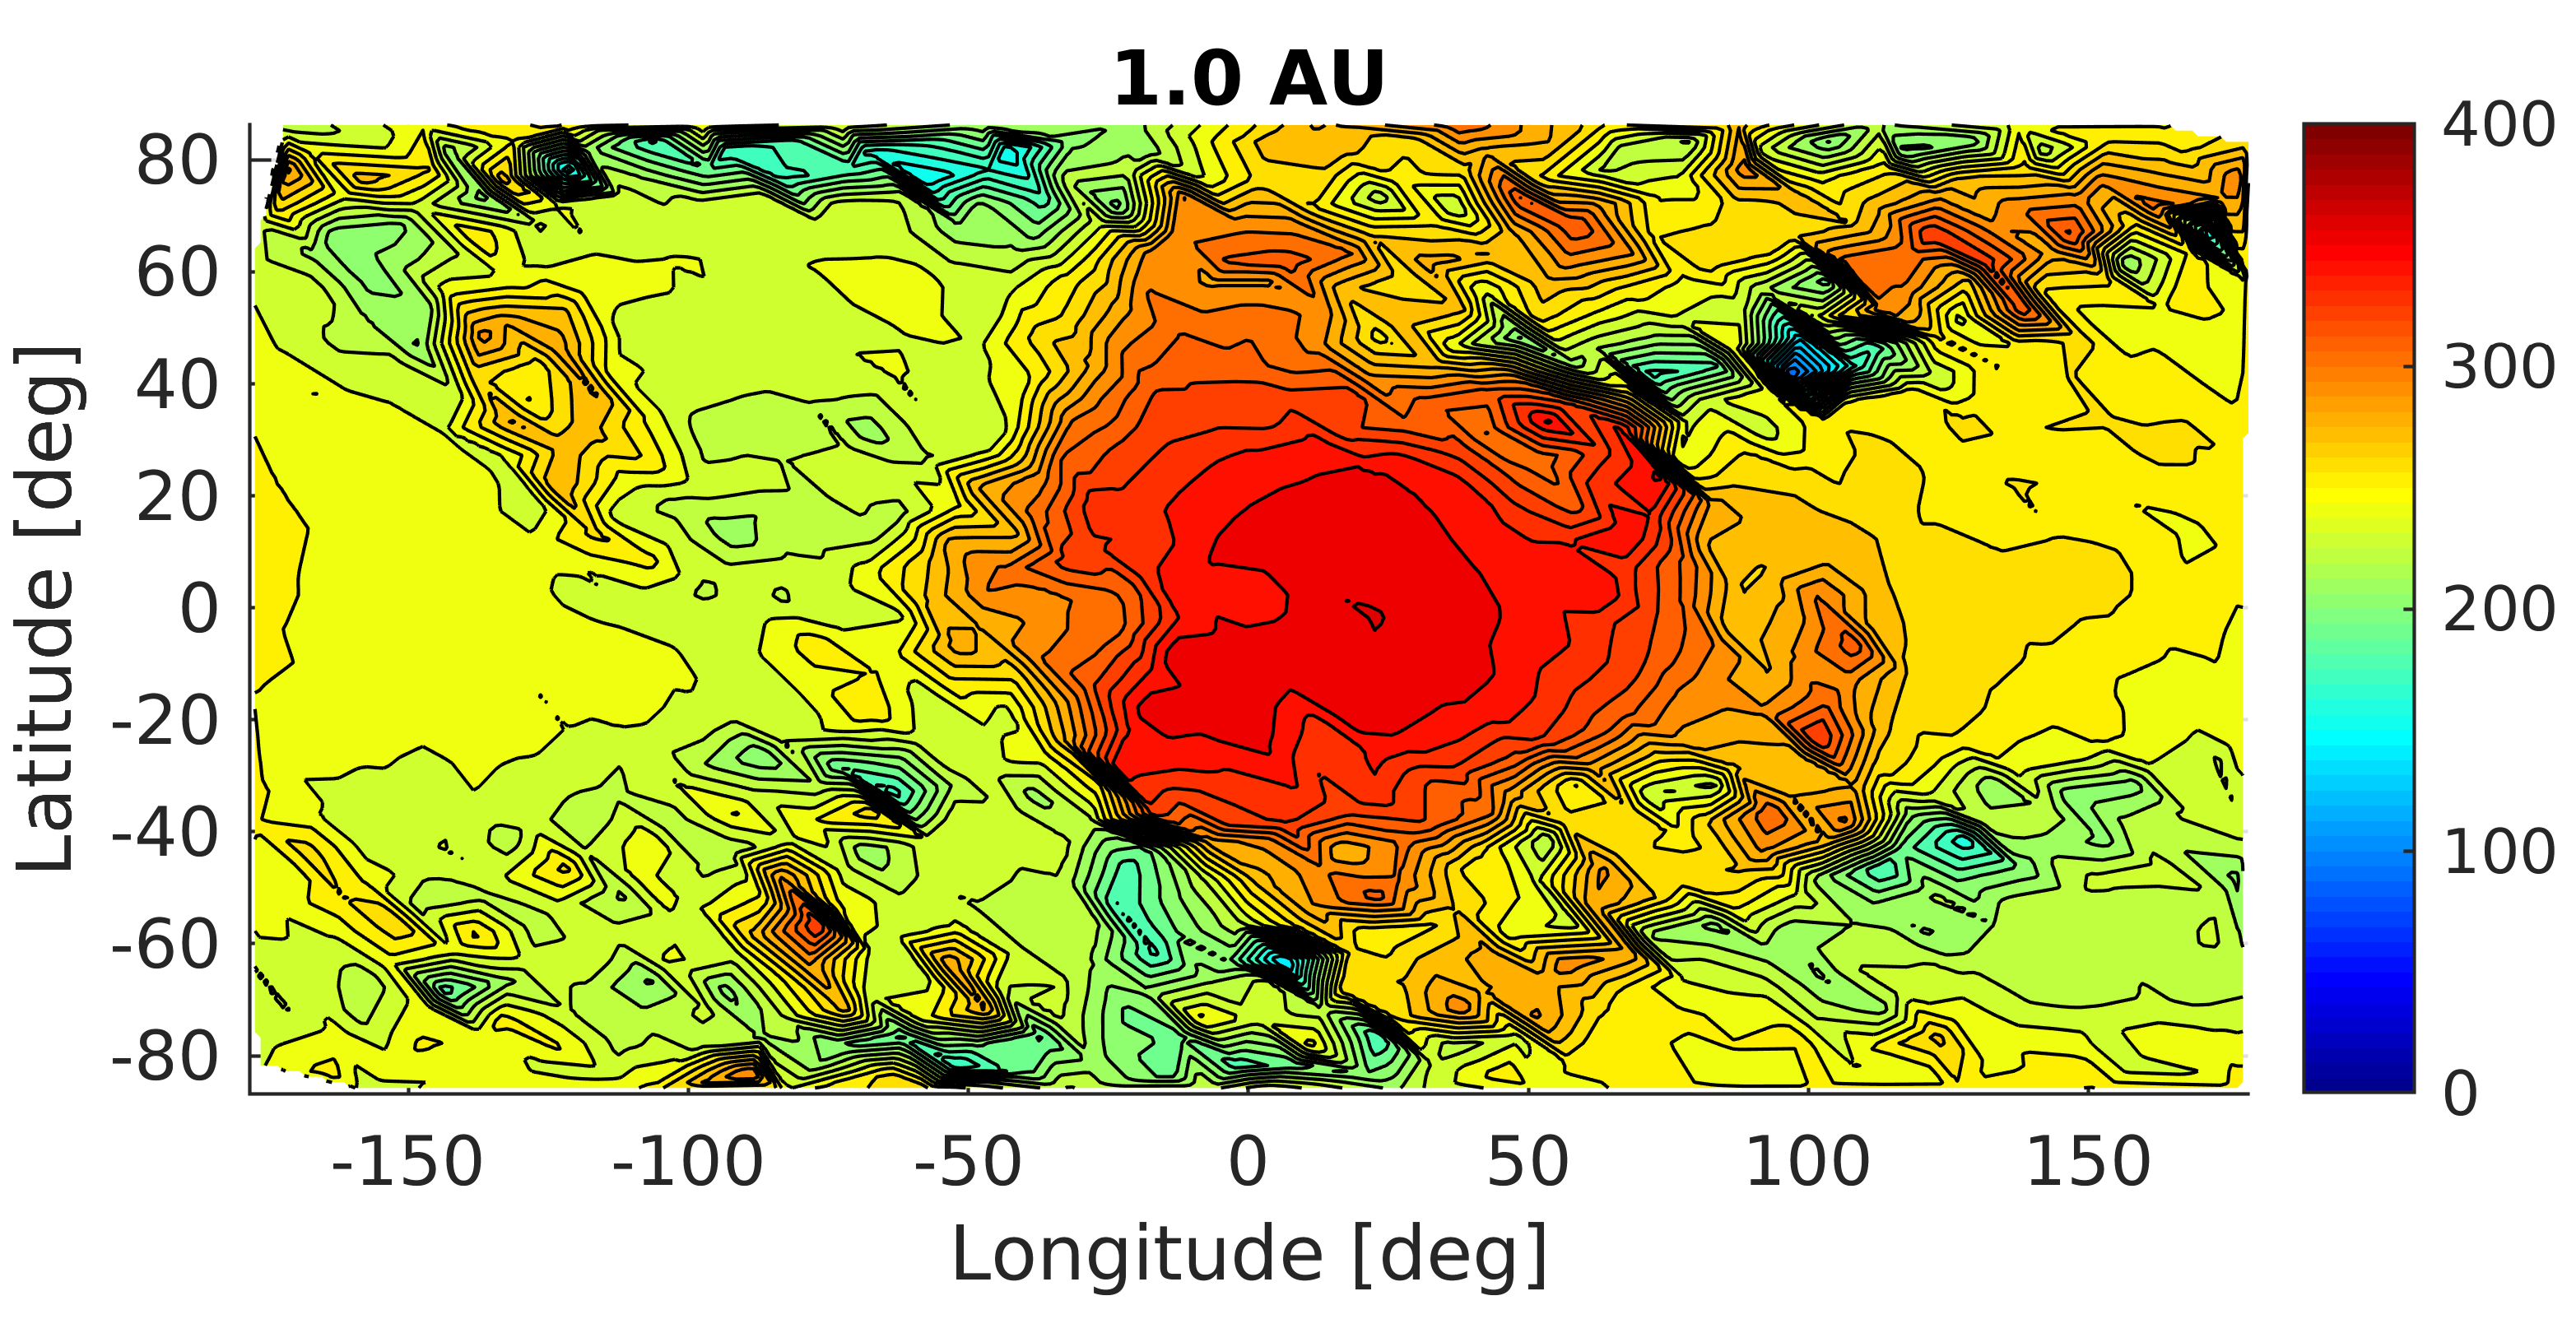
\includegraphics[width=\linewidth]{rsc/self_2D.png}
    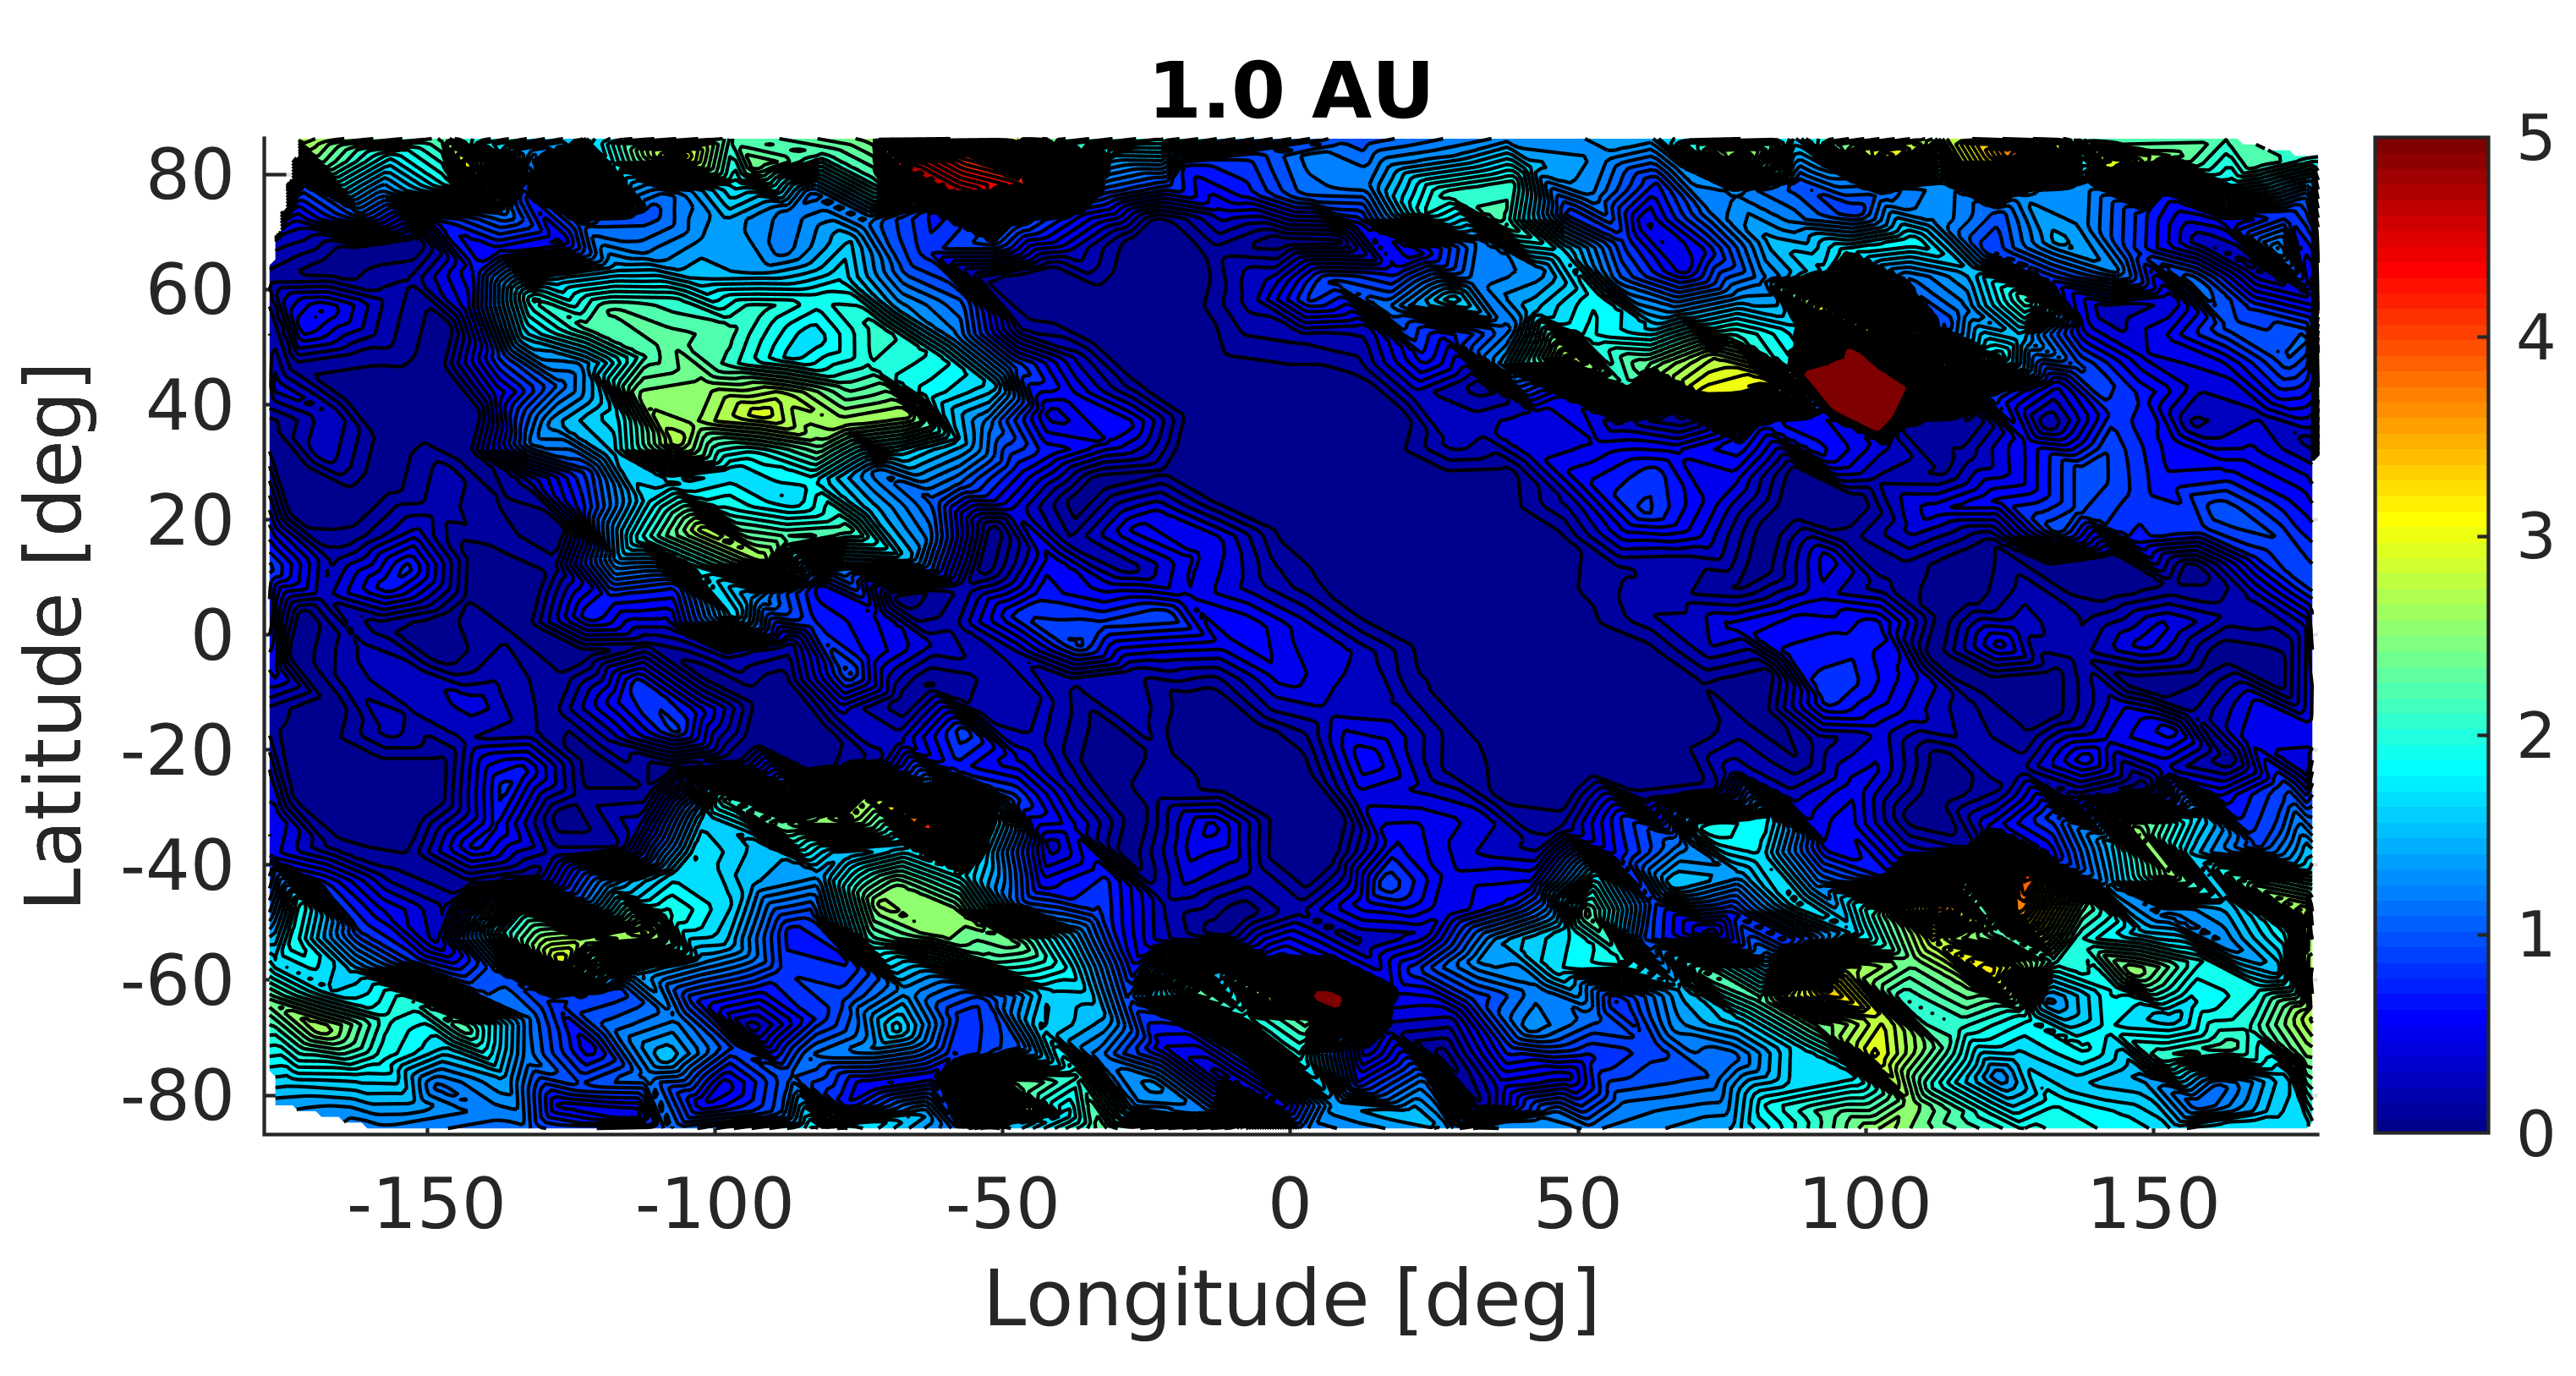
\includegraphics[width=\linewidth]{rsc/self_2D_diff.png}
    \captionof{figure}{The first figure is the thermal map of the surface of the asteroid Mathilde including its self heating. The second figure is the contribution of the self heating on thermal map. Orbital parameters and asteroid properties are taken as in \autoref{sec:4}.}
    \label{fig:5.3}
\end{center}

The contribution of the self heating may appear to be in some places higher than 5 Kelvins, as shown in \autoref{fig:5.4}, but this color axis has been chosen for reading purposes.
\begin{figure}
    \centering
    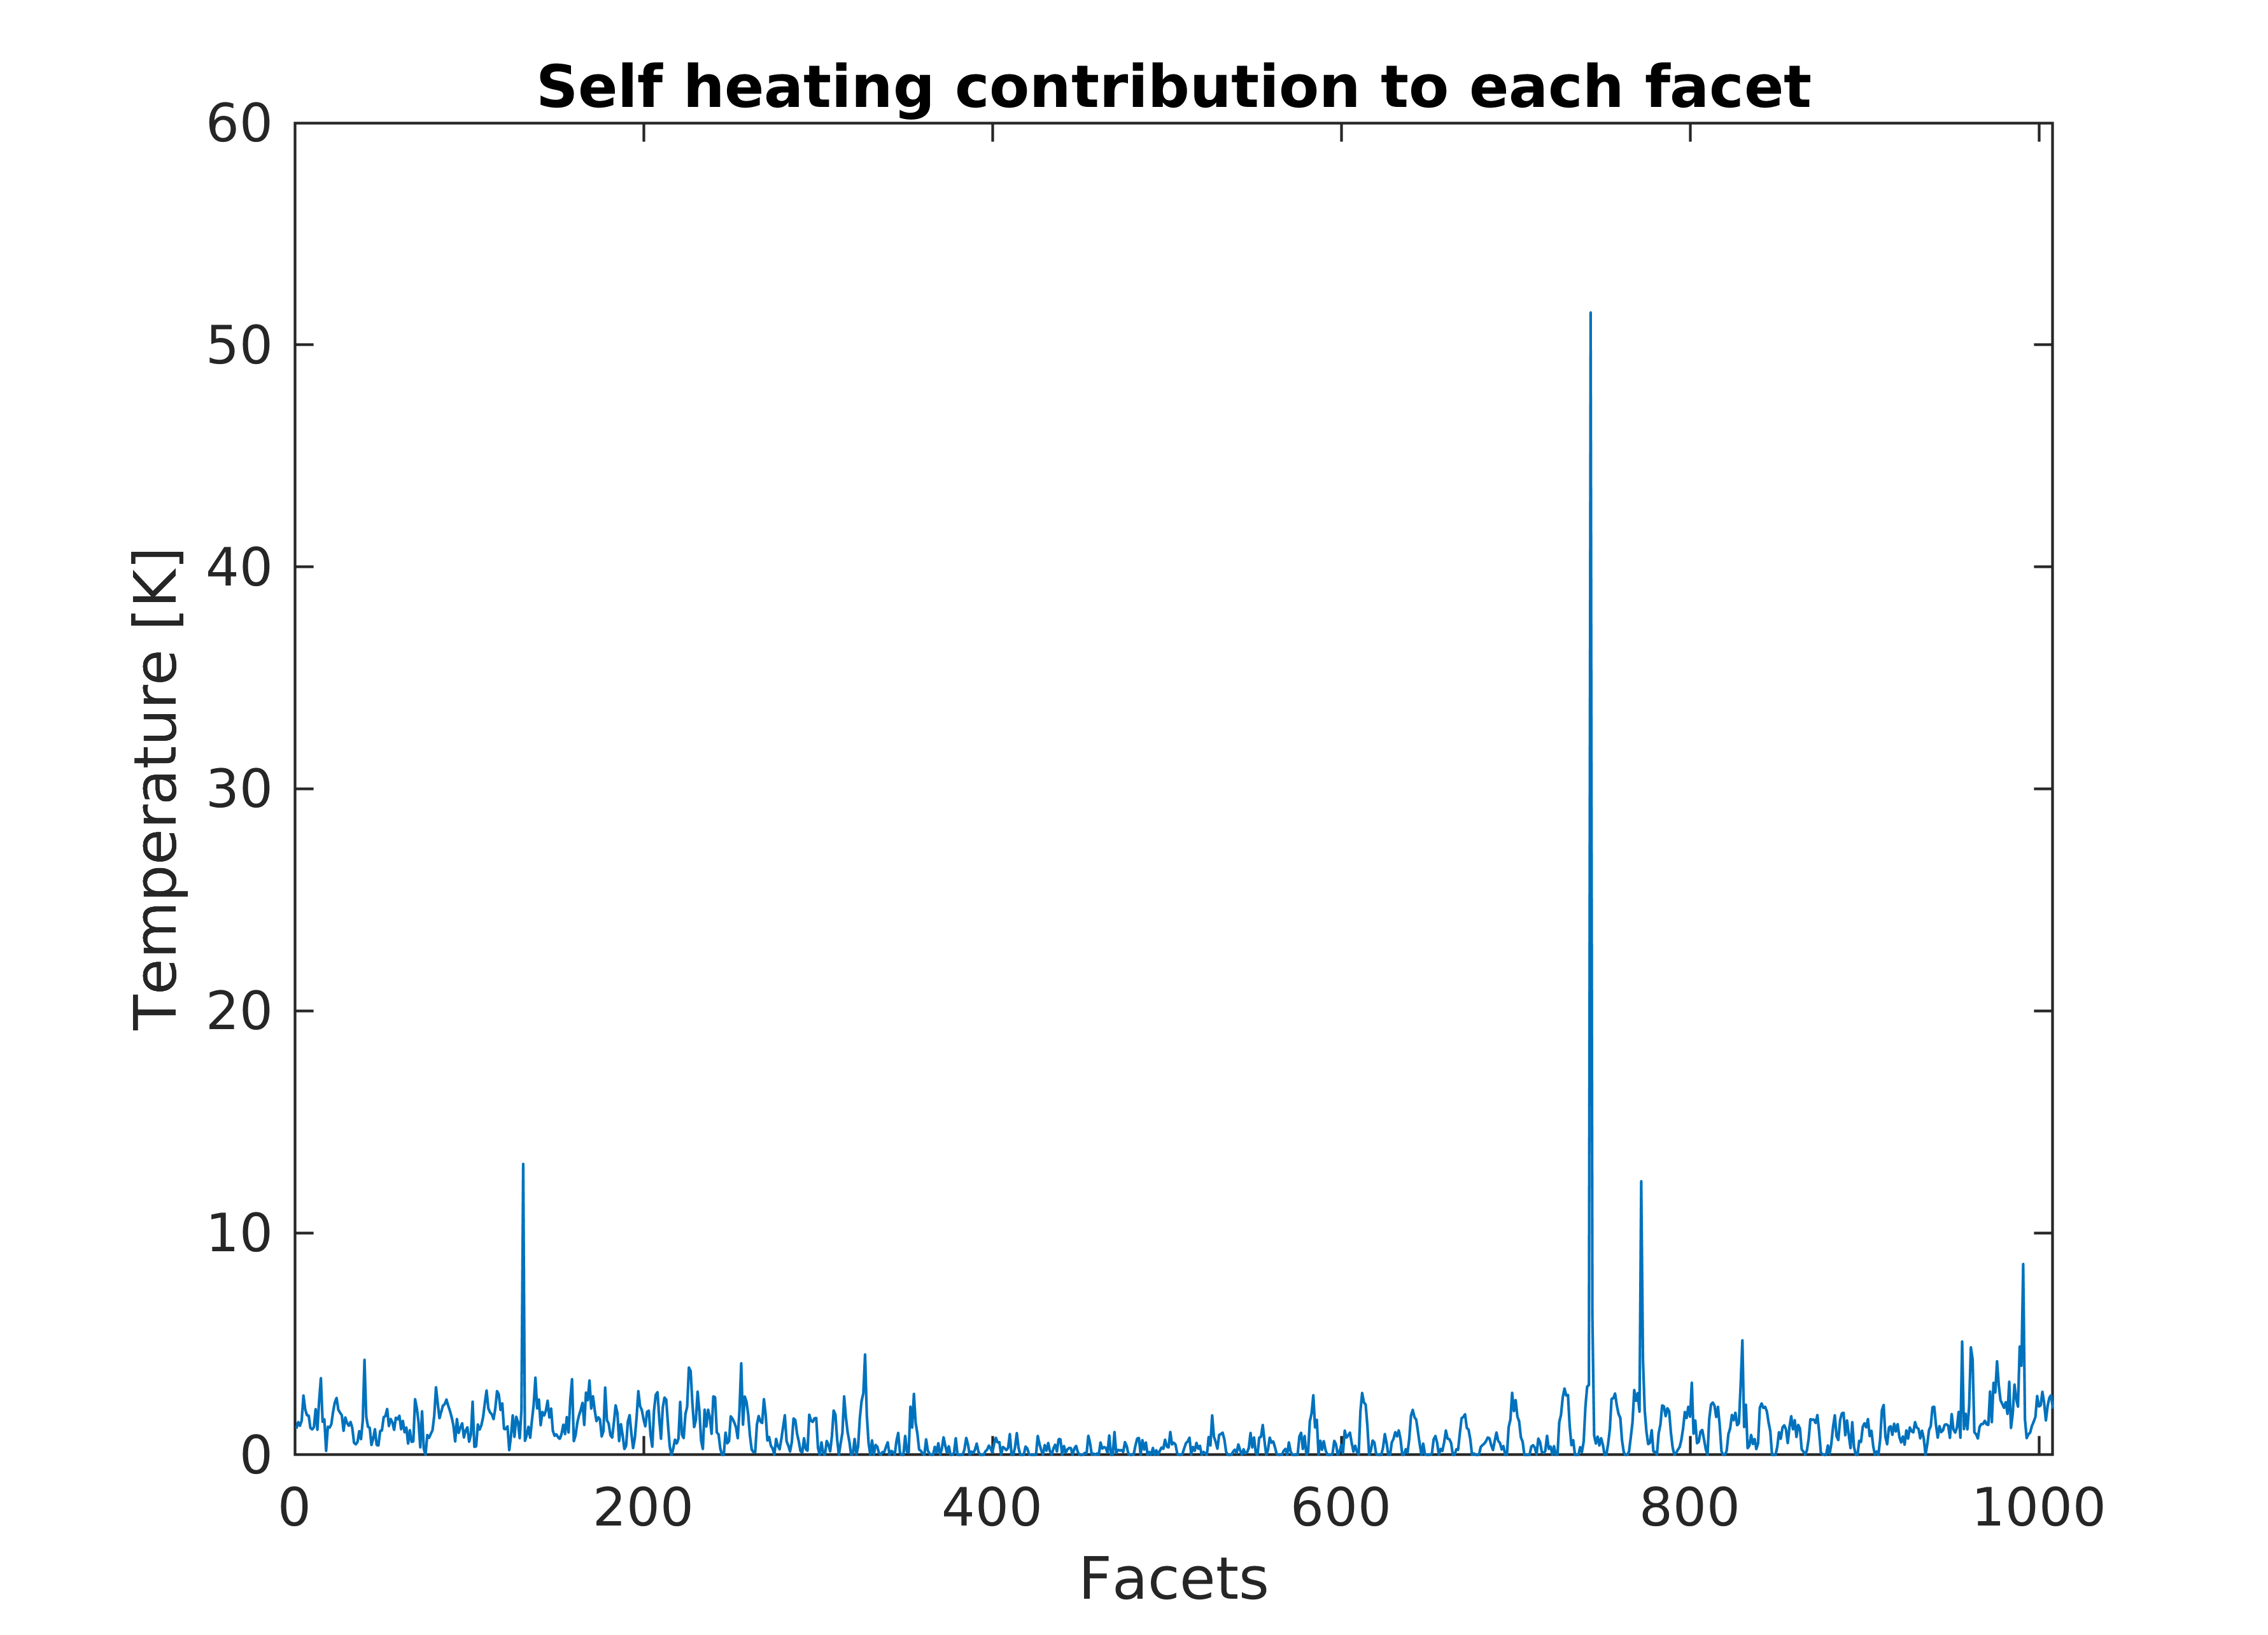
\includegraphics[width=\linewidth]{rsc/self_contribution.png}
    \caption{Distribution of the self heating contribution for each facet. Most values are located between 0 and 5 Kelvin.}
    \label{fig:5.4}
\end{figure}

Results in \autoref{fig:5.5} appear to be consistent. The self heating distribution of the contribution is mostly located in craters. The roughness of the asteroid also contributes in the creation of self heating.
